\documentclass{beamer}

\mode<presentation> {
%\usetheme{Berkeley}
%\usetheme{Frankfurt}
\usetheme{Madrid}
}
\usepackage[french]{babel}
\usepackage[T1]{fontenc}
\usepackage[utf8]{inputenc}
\usepackage{graphicx}
\usepackage{booktabs}

\hypersetup{
pdfauthor = {Jean Barré},
pdftitle = {Présentation mémoire de master 1 HN de l'Ecole des Chartes},
pdfsubject = {measuring literary value},
pdfkeywords = {Lecture distante} {Traitement automatique de la langue} {Canon littéraire} {Histoire Littéraire}
}

\title[Le prestige littéraire en lecture distante]{ENTRE CANON ET ARCHIVE, UNE ÉTUDE DES DYNAMIQUES TEXTUELLES À GRANDE ÉCHELLE.}

\author{Jean Barré}
\medskip

\institute[ENC]
{
École Nationale des Chartes
\medskip
\textit{jean.barre@chartes.psl.eu}
}
\medskip
\date{15 Décembre 2021}

%--------------------------------------------------------------------
%	PRÉSENTATION
%--------------------------------------------------------------------

\begin{document}

%------------------------------------------------
\begin{frame}
\titlepage
\end{frame}
%------------------------------------------------
\begin{frame}
\frametitle{Table des matières}
\tableofcontents
\end{frame}
%------------------------------------------------

\section{Introduction}
%------------------------------------------------

\begin{frame}
\frametitle{Introduction}

\begin{block}{Le canon littéraire}
Le canon est une règle, un modèle, une norme à imiter. Les études littéraires s’intéressent à cet ensemble qui ne représente qu’une partie infime de la production littéraire des siècles passés.
\end{block}

\begin{block}{La lecture distante\cite{p1}}
Concept que l'on doit à Moretti. Le but est d'explorer le passé littéraire (et ce qu'en dit la théorie et l'histoire littéraire) avec avec les méthodes computationnelles. Cela nous est rendu possible par la constitution de grand corpus d'ouvrages numérisés.
\end{block}

\begin{block}{Traitement Automatique des Langues}
La partie technique de mon mémoire se trouve dans l'implémentation de techniques du TAL pour parcourir les textes et en extraire les informations pertinentes. 
\end{block}

\end{frame}
%------------------------------------------------

\AtBeginSection[ ]
{
\begin{frame}{Le mémoire de M1}
    \tableofcontents[currentsection]
\end{frame}
}
%------------------------------------------------

\section{Le mémoire de M1}

\subsection{Enjeux et hypothèses}
%------------------------------------------------

\begin{frame}
\frametitle{Enjeux et hypothèses}
\begin{itemize}
\item Mettre au jour l'existence de dynamiques textuelles entre canon et non-canon.
\item Hypothèse d'une sélection successive des textes les plus informatifs au détriment d'une majorité d'autres.
\item Cette simplification nous permet de rentrer dans les textes avec des éléments quantifiables, comme par exemple la variété lexicale.
\item Travail fondé sur les recherches réalisés au Stanford Literary Lab, qui montraient des différences textuelles forte entre canon et non-canon\cite{p5}.
\end{itemize}



\end{frame}
%------------------------------------------------

\subsection{Le corpus de travail}
%------------------------------------------------

\begin{frame}
\frametitle{Corpus ANR Chapitres}
\begin{itemize}
\item 2968 romans du \textsc{XIX}\ieme ~et \textsc{XX}\ieme ~siècle
\item Équilibre entre les œuvres appartenant ou non au canon.
\end{itemize}
\begin{figure}
    \centering
    \includegraphics[width=10cm]{corpus_bar.png}
    \caption{Répartition du corpus dans le temps}
    \label{corpus_bar}
\end{figure}
\end{frame}
%------------------------------------------------

\subsection{Chaîne de traitement}
%------------------------------------------------

\begin{frame}
\frametitle{Chaîne de traitement}
\begin{columns}[c]

\column{.4\textwidth}
\textbf{Trois composantes majeures:}
\begin{enumerate}
\item Spacy
\item Stylométrie roulante
\item Entropie et Type-token ratio
\end{enumerate}

\column{.6\textwidth}
\begin{figure}
    \centering
    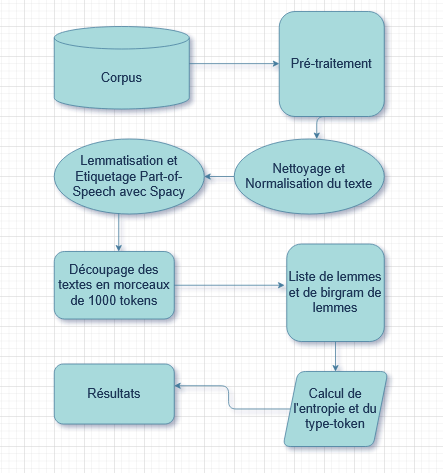
\includegraphics[width=6cm]{00_workflow_final.png}
    \caption{Chaîne de traitement}
    \label{workflow}
\end{figure}

\end{columns}
\end{frame}
%------------------------------------------------


\begin{frame}{Les mesures}

\begin{theorem}[Entropy]
\begin{equation}
H\ensuremath{\prime}=-\sum_{i=1}^R pi ln pi
\end{equation}
\end{theorem}
\begin{theorem}[Type-token ratio]
\begin{equation}
TTR = 100 * nb types / nb tokens
\end{equation}
\end{theorem}

\end{frame}
%------------------------------------------------

\subsection{Visualisation des résultats}
%------------------------------------------------

\begin{frame}
\frametitle{Visualisation des résultats - 1/2}
\begin{figure}
    \centering
    \includegraphics[width=12cm]{regression_entropy.png}
    \caption{Mesure de la redondance des bigrammes}
    \label{entropy}
\end{figure}
\end{frame}

%------------------------------------------------

\begin{frame}
\frametitle{Visualisation des résultats - 2/2}
\begin{figure}
    \centering
    \includegraphics[width=12cm]{regression_type_token.png}
    \caption{Mesure de la redondance des lemmes}
    \label{type_token}
\end{figure}
\end{frame}
%------------------------------------------------


\subsection{Analyse des résultats}
%------------------------------------------------

\begin{frame}
\frametitle{Analyse des résultats}
\begin{itemize}
    \item Nous n'obtenons pas les mêmes résultats que dans l'étude du Literary Lab. 
    \item L'hypothèse n'est pas validée empiriquement.
    \item On constate une démarcation de nos deux groupes de textes sur une période de 50 ans.
    \item Les textes canoniques connaissent une hausse de redondance sur cette période. Comment interpréter cela ?
\end{itemize}

\end{frame}

%------------------------------------------------
\subsection{Conjectures}
%------------------------------------------------

\begin{frame}
\frametitle{Conjectures}
\begin{columns}[c]

\column{.4\textwidth}
\textbf{Les mesures détecteraient le Nouveau Roman :}
\begin{enumerate}
\item La situation temporelle correspond
\item Registre de langue familier
\item Oralité du discours
\end{enumerate}

\column{.6\textwidth}
\begin{figure}
    \centering
    \includegraphics[width=7cm]{nouveau_roman.png}
    \caption{Redondance dans les romans canoniques}
    \label{new_roman}
\end{figure}

\end{columns}
\end{frame}
%------------------------------------------------

\AtBeginSection[ ]
{
\begin{frame}{Les recherches en cours}
    \tableofcontents[currentsection]
\end{frame}
}

\section{Les recherches en cours}

\subsection{Constats et Limites du mémoire de M1}
%------------------------------------------------

\begin{frame}
\frametitle{Constats et Limites du mémoire de M1}

\begin{itemize}
    \item Le corpus Chapitres désigne un texte comme étant canonique à partir du nombre de résultats d'une requête sur fabula.org.
    \item La canonicité est définie de manière binaire à l'échelle des auteurs et non des ouvrages.
    \item Une hypothèse (le canon littéraire est peu redondant - plus informatif) un peu légère pour saisir des liens potentiels entre une réalité textuelle et les contextes de la production littéraire.
\end{itemize}

\end{frame}
%------------------------------------------------

\subsection{Définir un Canon Littéraire}
%------------------------------------------------

\begin{frame}
\frametitle{Définir un Canon Littéraire}
\begin{itemize}
    \item Le prestige littéraire comme probabilité qu'un auteur soit discuté, étudié et enseigné dans le champ littéraire\cite{p7} contemporain.
    \item Pour identifier cela je détermine un indice de canonicité entre 0 et 1, qui décrit à quel point un texte est canonique. 
\end{itemize}

\textbf{Plusieurs paramètres à cet indice : }

\begin{enumerate}
\item Publication en oeuvre complète aux éditions de la Pléiade.
\item Publication avec appareil critique aux éditions Gallimard-Flammarion
\item Récupération des listes des textes au programme de l'agrégation depuis 1969
\item Nombre de citation dans le Lagarde et Michard
\end{enumerate}

\end{frame}
%------------------------------------------------


\subsection{Formaliser la Littérarité}
%------------------------------------------------

\begin{frame}
\frametitle{Formaliser la Littérarité}
\begin{block}{Concept de littérarité}
Ce qui constitue le discours littéraire.\cite{p4} L'idée est de détecter et de décrire les traits formels d'une esthétique littéraire.
\end{block}

\begin{block}{Hypothèse}
 La littérarité d'un texte est un des critères de sélection des chercheurs en littérature pour déterminer si un texte vaut la peine d'être étudier. Cela expliquerait la persistance temporelle des textes.
\end{block}

\textbf{Littérarité formelle : }

\begin{enumerate}
\item Longueur des phrases.
\item Complexité syntaxique des phrases.
\item Distribution lexicale des textes.
\item Détection des stylèmes, fondés sur les mots outils
\end{enumerate}
\end{frame}
%------------------------------------------------

\subsection{Modéliser et Prédire la Canonisation}
%------------------------------------------------

\begin{frame}
\frametitle{Modéliser et Prédire la Canonisation}

\begin{itemize}
    \item Recherche de corrélations entre littérarité et prestige littéraire.
    \item Entraîner un modèle statistique (SVM) sur les caractéristiques textuelles de la littérarité.
    \item Comparer les résultats des deux approches, entre les contextes et les caractéristiques textuelles des textes. 
\end{itemize}

\end{frame}
%------------------------------------------------

\section{Conclusion}
%------------------------------------------------

\begin{frame}
\frametitle{Conclusion}
\begin{itemize}
    \item Je cherche si les textes étudiés par les chercheurs successifs ont une composante textuelle qui les démarquent au sein de la production littéraire.
    \item Je cherche si le phénomène social de la reconnaissance littéraire est en relation avec un type particulier d'écriture. 
\end{itemize}

\textbf{Pistes de réflexion :}
\begin{itemize}
    \item Enrichir mon corpus de texte avec le contexte contemporain de réception.
    \item Questionner les standards du jugement esthétique et leur évolution au cours du temps.
    \item Entraîner plusieurs modèles sur plusieurs périodes de réception. 
    \item Revenir à une lecture proche : Les morceaux de texte que le modèle considère comme le plus littéraire.
\end{itemize}

\end{frame}

%--------------------------------------------

\begin{frame}
\frametitle{Bibliographie indicative}
\footnotesize{
\begin{thebibliography}{99}

\bibitem[Moretti, 2013]{p1} Franco Moretti (2013)
\newblock Distant reading

\bibitem[Underwood, 2019]{p2} Ted Underwood (2019)
\newblock Distant horizons: digital evidence and literary change

\bibitem[Philippe, 2009]{p3} Gilles Philippe, Julien Piat (2009)
\newblock La langue littéraire: une histoire de la prose en France de Gustave Flaubert à Claude Simon

\bibitem[Molinié, 1993]{p4} Georges Molinié, Alain Viala (1993)
\newblock Approches de la réception

\bibitem[Hewitt, 2016]{p5} M. Algee-Hewitt, S. Allison, M. Gemma, R. Heuser, F. Moretti and H. Walser. (2016)
\newblock Canon/Archive, Large scale dynamics in the literary field

\bibitem[Guillory, 1998]{p6} John Guillory (1998)
\newblock Cultural capital: the problem of literary canon formation

\bibitem[Bourdieu, 1992]{p7} Pierre Bourdieu (1992)
\newblock Les règles de l'art : Genèse et structure du champ littéraire

\end{thebibliography}

}
\end{frame}

%--------------------------------------------------------------------------------

\end{document} 